\section{Анализ предметной области}
%Тема - Интеллектуальная система мониторинга и распознавания загрязнений водоемов
%написать про методы распознавания разливов иишками, их плюсы и минусы
%примерная структура - разливы, способы мониторинга, нейронки (и их исследование)
\subsection{Актуальность проблемы загрязнения водоемов}

Вода является одним из важнейших природных ресурсов, как для поддержания жизнедеятельности биологических систем, так и для обеспечения разнообразных промышленно-технологических процессов.  Сегодня вода активно используется в различных ключевых отраслях. В металлургии вода применяется в процессах флотации - обогащения различных руд, а также для охлаждения доменных печей. Химическая промышленность активно задействует воду  для очищения и охлаждения оборудования на различных нефтеперерабатывающих производствах, как компонент для создания продуктов нефтехимической отрасли, таких как пластмассы, реагенты и растворители, удобрения. Вода также активно применяется как один из материалов для создания фармацевтической продукции, такой как инъекционные растворы, препараты для наружного применения(спреи и капли).  Энергетический сектор также использует воду для охлаждения энергетического оборудования на атомных и теплоэлектростанциях. Кроме того, вода так же обеспечивает работу гидроэлектростанций. 

 Загрязнение водоемов негативно сказывается на экологии, здоровье населения, препятствует развитию экономики, поэтому обеспечение экологической безопасности водоемов является одной из наиболее важных задач экологии. В настоящее время особую актуальность приобретает проблема нефтяных разливов.
 
\subsection{Нефтяные разливы}

\subsubsection{Экологическая опасность нефтяных разливов}
%частота разливов, крупные трагедии, причины разливов (то есть не только транспорт)
Разлив нефти -- аварийный выброс нефти или нефтепродуктов в окружающую среду. Нефтяные разливы происходят с высокой частотой и являются серьезной проблемой нефтегазовой отрасли. Каждый разлив приводит к масштабным последствиям для окружающей среды и требует значительных финансовых затрат для устранения самого разлива и минимизации экологического ущерба. 

Ярким примером является инцидент на буровой платформе Deepwater Horizon, принадлежавшей британской нефтегазовой компании British Petrolium. 20 апреля 2010 года, в результате нарушения технологических норм цементирования скважины, произошел взрыв, который привел к гибели 11 человек и неконтролируемому выбросу нефти в Мексиканский залив на протяжении нескольких месяцев. В окружающую среду попало около 400 тысяч тонн нефти. Эта катастрофа, ставшая крупнейшим в истории США разливом нефти, привела к массовой гибели животных, таких как дельфины, морские черепахи, тем самым нанеся колоссальный ущерб морским экосистемам, по некоторым оценкам сохраняющийся и по сей день. Расходы на ликвидацию происшествия, а также затраты на штрафы и компенсации, составили около 65 миллиардов долларов.

16 марта 1978 года французский супертанкер Amoco Cadiz, попав в шторм, потерял управление и разбился о скалы у берегов французского региона Бретань. Это происшествие привело к выбросу 220 тысяч тонн сырой нефти в Атлантический океан, загрязнив более 300 километров французского побережья. Пролившаяся нефть образовала пятно протяженностью 19 километров и поникла в песок на глубину до 50 сантиметров, образовав асфальтоподобные корки, сохранявшиеся на протяжении нескольких лет. В защищенных от волн районах нефть сохранялась до 10 лет, тем самым замедляя восстановление экосистемы, понесшей масштабный ущерб -- загрязнение вызвало гибель около 20 тысяч птиц, множества донных организмов, таких как моллюски и ракообразные. Рыбаки сообщали о сокращении уловов в два раза, а сама рыба нередко имела различные язвы и опухоли. Компания Amoco, владелец танкера, выплатила Франции компенсацию в размере 230 миллионов долларов.

Не менее разрушительными оказались последствия крушения танкера Prestige, затонувшего в ноябре 2002 года. Получив повреждения у побережья Испании, корпус судна раскололся, что привело к попаданию примерно 60 тысяч тонн нефти в Атлантический океан. Растянувшееся на более чем 2000 километров вдоль побережья Галисии нефтяное пятно поставило под угрозу существование 25 охраняемых видов животных, уничтожило популяции рыб, кораллов, моллюсков. Согласно государственной оценке, зачистка побережья Галисии обошлась в 2,5 миллиарда евро, а нанесенный ущерб составил 368 миллионов евро. 

В июле 2010 года нефтепровод, принадлежащий американской корпорации Enbridge, разорвало в результате коррозии трубы, что послужило причиной попадания более 2,7 тонн битумной нефти в реку Каламазу, пролившейся на 40 километров по руслу реки и осевшей на дне. Осевшая нефть отравила донные отложения реки, что привело к массовой гибели рыб, популяции которых начали возвращаться только спустя 10 лет. Кроме того, токсины сделали речную воду непригодной для питья, а из-за ядовитых испарений нефти некоторые жители близлежащих районов жаловались на головные боли и тошноту.  Поскольку убирать пролившуюся нефть пришлось не только с поверхности, но и со дна реки, очистные мероприятия были значительно затруднены, что повысило стоимость их проведения -- она составила примерно 1,2 миллиарда долларов.

Утром 15 декабря 2024 года в Керченском проливе в результате шторма танкеры <<Волгонефть-212>> и <<Волгонефть-239>>, перевозившие в общей сложности около 9000 тонн мазута, потерпели крушение. По различным оценкам в море попало от 2,5 до 5 тысяч тонн мазута, разлившегося по площади более 400 м$^{2} $. Загрязнение затронуло около 70 километров береговой линии и привело к гибели более 200 птиц и 70 дельфинов, среди которых были охраняемые виды. Реагируя на происшествие, власти вели режим чрезвычайной ситуации на федеральном уровне и объявили о начале масштабных очистных работ с участием 300 человек и 60 единиц специальной техники, продолжающихся по сей день.

Вследствие принятия множества международных законов и соглашений, совершенствования технологических процессов можно отметить уменьшение частоты крупных происшествий, приводящих к масштабным разливам нефти. Однако, некоторые исследования\cite{spill_db} отмечают, что информация о разливах нефти не всегда достоверна, утверждая, что многие менее крупные инциденты никогда не попадают в поле зрения государственных служб контроля и СМИ, что приводит к отсутствию данных об этих инцидентах в международных и государственных базах. 

\subsubsection{Причины и источники загрязнений}
Основными источниками разливов нефти являются различные утечки на этапах добычи, хранения и транспортировки нефти и нефтепродуктов. Причинами возникновения утечек могут являться как стихийные бедствия, такие как штормы, землетрясения и эрозия, так и техногенные факторы, включая отказы оборудования, человеческие ошибки.  В таблице 1.1 указаны основные источники попадания нефти в мировой океан\cite{spill_reasons}.

\begin{xltabular}{\textwidth}{|l|l|p{3.2cm}|X|}
	\caption{Основные источники попадания нефти в мировой океан\label{oil_source:table}}\\ \hline
	Источник & млн. т/год \\ \hline
	\endfirsthead
	\continuecaption{Продолжение таблицы \ref{oil_source:table}}\\ \hline
	Источник & млн. т/год \\ \hline
	\endhead
	Морская транспортировка (кроме аварийных разливов) & 1,83 \\ \hline
	Аварийные разливы & 0,3 \\ \hline
	Речной сток, включая сточные воды городов & 1,9 \\ \hline
	Сточные воды прибрежной зоны & 0,8 \\ \hline
	Естественные нефтяные скважины & 0,6 \\ \hline
	Добыча нефти в море & 0,08 \\ \hline
	Всего & 5,51 \\ \hline
\end{xltabular}

Наиболее часто разливы нефти появляются в результате аварии на танкере, перевозящем нефть или нефтепродукты. Среди причин возникновения таких аварий можно выделить столкновения, посадки на мель, штормовые повреждения, нарушение герметичности резервуаров. Эти происшествия нередко приводят к масштабным выбросам нефти в морскую или речную среду, при этом загрязняя не только воду, но и зачастую прибрежные зоны, в районе которых произошла авария.
 
Морская добыча нефти проводится с помощью масштабных комплексов, использующих комплекс инженерно-технических решений. Такие происшествия, как повреждения герметизации скважин, отказ оборудования, ошибки при цементировании или нарушения технологических регламентов приводят к выбросам добываемой нефти из подземных резервуаров, что в свою очередь приводит к разливам, плохо поддающимся локализации.

Трубопроводы, используемые для транспортировки нефти на большие расстояния, могут дать течь вследствие коррозии труб, механических повреждений, ошибок в обслуживании. В результате в воде может образоваться нефтяной разлив, который может долго оставаться незамеченным, если трубопровод проходит под водой. Кроме того, серьезную угрозу загрязнения представляет преднамеренное разрушение нефтяной инфраструктуры, особенно в зонах активных боевых действий. Атаки на эти объекты не только приводят к масштабным утечкам, но и затрудняют обнаружение и ликвидацию последствий разливов.

Промышленные предприятия, связанные с переработкой нефти, могут сбрасывать загрязненные нефтью или продуктами ее переработки воды в близлежащие водоемы. Наряду с этим отходы ремонтных мастерских, автозаправочных станций также могут попадать в водоемы, что приводит к еще большему загрязнению.

Нефтяные утечки происходят не только по вине человека, но и в ходе естественного просачивания из нефтеносных пластов земли через трещины в коре. Чаще всего это происходит в районах активной геологической активности. Несмотря на относительно незначительные объемы, эти утечки также оказывают негативное влияние на экосистемы.

\subsection{Методы мониторинга разливов нефти}

Своевременное обнаружение и ликвидация нефтяных разливов -- ключевые задачи для сохранения экологической безопасности водоемов. В связи с этим широко распространены различные виды мониторинга состояния водоемов. среди которых выделяются визуальные методы наблюдения за поверхностью воды. В отличие от лабораторных исследований, визуальное исследование позволяет намного быстрее охватить большие территории и не требует физического контакта с объектом, что позволяет оперативно обнаружить новые разливы нефти, особенно в труднодоступных акваториях. 

Одним из самых распространенных методов визуального мониторинга является спутниковая съемка. Современные спутники, оснащенные высокоточными сенсорами, позволяют получить качественные снимки поверхности воды и хорошо отображают аномалии, такие как нефтяные пятна. Спутниковая съемка охватывает сотни квадратных километров поверхности Земли в одном снимке, а использование групп спутников позволяет получать новые данные с высокой периодичностью. Кроме того, использование многих спутников бесплатно, а данные размещены в открытом доступе, что снижает стоимость процедур мониторинга. Однако, зависимость космической съемки от погодных условий и времени суток значительно осложняет наблюдение за поверхностью водоемов и является существенным недостатком этого метода.

В условиях плохой видимости, ограничивающих работу спутников, применяются радиолокационные спутниковые снимки. В отличие от оптических сенсоров, радары полагаются на электромагнитные сигналы и фиксирую отраженный поверхностью воды отклик, что и позволяет вести съемку в любую погоду и время суток. На радарных снимках нефтяные пятна обычно проявляются в качестве темных областей, что повышает их информативность в задачах обнаружения нефтяных пятен и пленок.  Так, исследование радиолокационных снимков Керченского пролива с использованием спутников Sentinel-1A/B за период с 2017 по 2021 годы показало высокую точность этого метода и позволило исследовать частоту появления, масштаб нефтяных разливов и их источники на основании 2597 пятен, появившихся на снимках за этот период\cite{radiophoto}. Несмотря на гибкость этого метода, полученные снимки нередко проявляют сторонние объекты, например различные биологические образования, создавая визуально похожие участки на изображениях. Наличие таких ложных данных требует участия эксперта, отличающего действительные нефтяные пятна от схожих объектов, в процессе мониторинга. Кроме того, радиолокационные изображения значительно дороже, что еще больше повышает стоимость мониторинга.

Наконец, высокую эффективность показал метод аэросъемки поверхностей воды. Вместе с развитием беспилотных летательных аппаратов, или БПЛА, наблюдение за водоемами с малой высоты стало высокоэффективным и экономически оправданным методом мониторинга. БПЛА часто оснащаются камерами высокого разрешения, что позволяет получать самые качественные снимки из перечисленных методов, а высокая степень гибкости в построении маршрутов и простота управления делают этот метод самым доступным. Недостатками аэросъемки с помощью БПЛА являются ограниченность радиуса и времени полета, что делает его малоэффективным для мониторинга больших поверхностей воды, таких как моря. Беспилотные аппараты часто используются в составе систем мониторинга вместе с спутниковыми системами для уточняющих съемок в определенных секторах, снимки которых получены из космоса. 

Перечисленные выше дистанционные методы используются для получения визуальных данных, являющихся источником информации для обнаружения нефтяных разливов. Чтобы обнаружить загрязнение, необходимо проанализировать полученные данные. Учитывая высокое количество изображений, полученных для анализа, этот процесс занимает значительное время. Более того, если изображения получаются в режиме реального времени, например в формате видеосъемки, то для обнаружения разлива нефти необходимо постоянное присутствие наблюдателя. В настоящее время для задач анализа изображений все чаще используются нейронные сети.

\subsection{Нейронные сети}
 
 \subsubsection{История появления нейронных сетей}
 
 Идеи, которые легли в основу современных нейронных сетей, берут свое начало в философии и математике, а основные принципы исследовались задолго до появления вычислительных систем как таковых. Правила, руководящие рациональной частью мышления были сформированы Аристотелем в далеких 384 -- 322 годах до нашей эры. Впоследствии формальные правила рассуждений и процессы мышления стали предметом исследований не менее известных философов, среди которых были Томас Гоббс (1588-1679),  Рене Декарт (1596-1650) и Рудольф Карнап (1891-1970)\cite{nn_history}. Известные математики, такие как Джордж Буль (1815-1864) и Готтлоб Фреге (1848-1925), внесли вклад в разработку логических систем, впоследствии ставших источниками исследований моделирования искусственного интеллекта. 
 
 Первая модель искусственного нейрона была предложена Уорреном МакКаллоком и Уолтером Питтсом в 1943 году. Модель представленного ими логического устройства показана на рисунке~\ref{fig:neuron}.
 
 \begin{figure}[h]
	\centering
	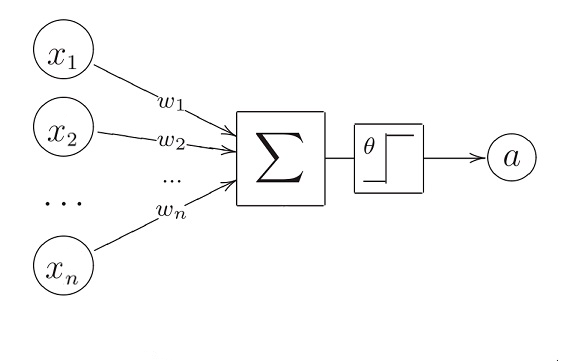
\includegraphics[width=0.7\linewidth]{images/neuron}
	\caption[]{Искусственный нейрон}
	\label{fig:neuron}
\end{figure}

Модель состоит из входов x$_{1}$, x$_{2}$, ... , x$_{n}$, весов w$_{1}$, w$_{2}$, ... , w$_{n}$, сумматора и функции активации. Попадая на входы, каждое значение x$_{i}$ умножается на значение соответствующего веса w$_{i}$, обозначающего его важность, после чего поступает на сумматор, вычисляющий сумму всех поступивших на него сигналов:
\[
z = w_1 x_1 + w_2 x_2 + \cdots + w_n x_n
\]
Полученная сумма затем сравнивается с пороговым значением θ. Если сумма больше, то нейрон возбуждается (выходное значение а = 1), в противном случае остается в состоянии покоя (выходное значение а = 0). Данная модель может выполнять только бинарные операции, получая на вход значения 0 и 1, требует ручного задания весов, также являющихся бинарными, и порогового значения, что значительно ограничивает её возможности. 

Несмотря на ограничения, предложенный МакКаллоком и Питтсем искусственный нейрон показал способность выполнять базовые логические операции, такие как И, ИЛИ и НЕ. Эта модель стала основой для дальнейшей теории нейронных вычислений, а все современные нейронные сети состоят из доработанных версий оригинальных нейронов. 

 Спустя несколько лет идеи, взяв за основу исследования МакКаллока и Питтса, американский ученый Фрэнк Розенблатт предложил схему перцептрона - устройства, моделирующего восприятие информации головным мозгом человека. Перцептрон состоит из входных датчиков, ассоциативных и реагирующих элементов\cite{perceptron}. Схема простейшего перцептрона показана на рисунке~\ref{fig:simpleperceptron}.
 
\begin{figure}[h]
	\centering
	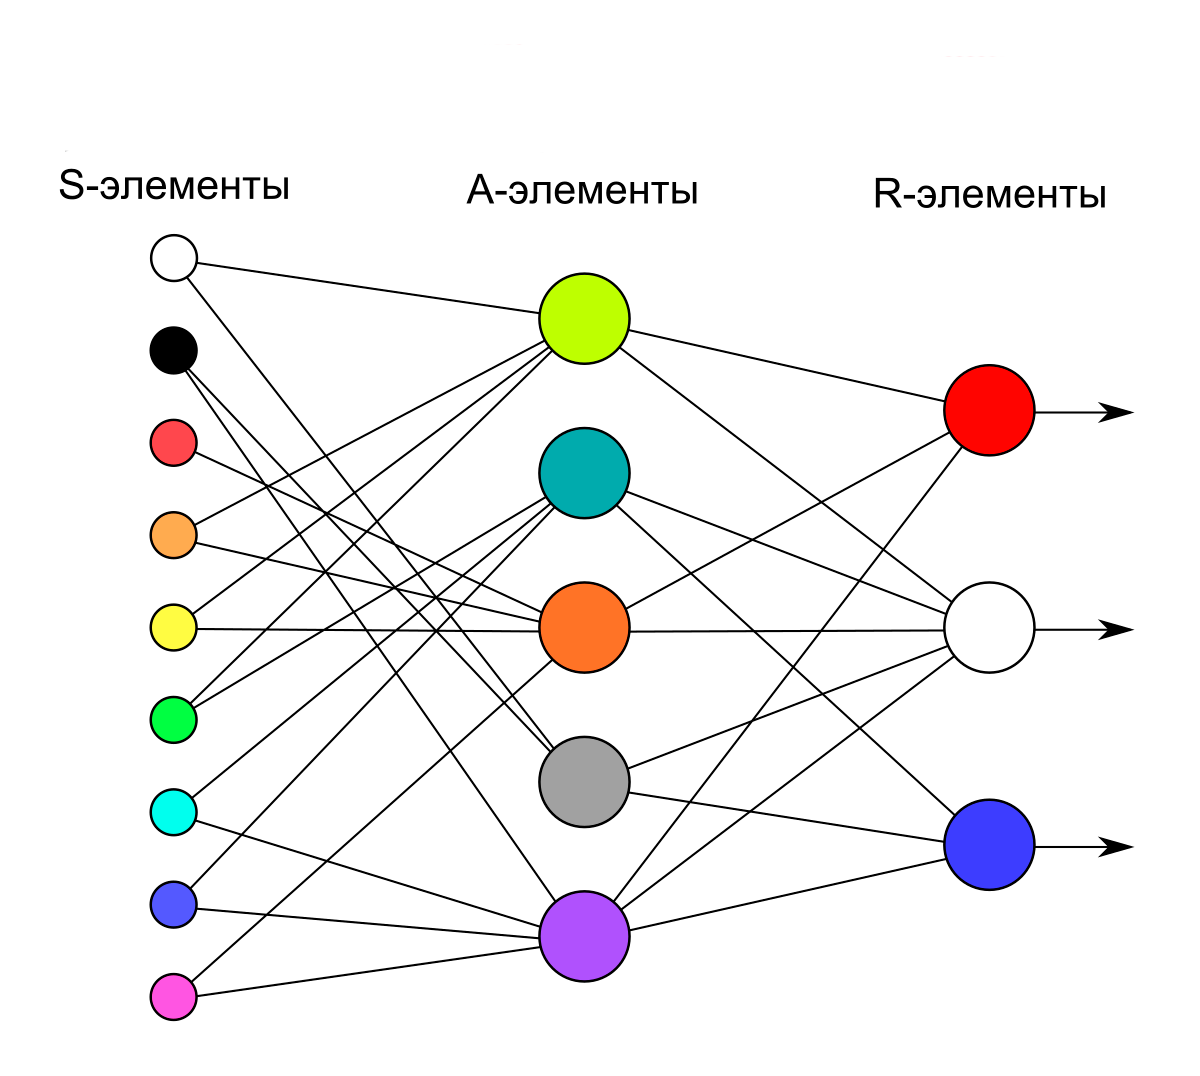
\includegraphics[width=0.7\linewidth]{images/Simple_perceptron}
	\caption{Схема однослойного перцептрона}
	\label{fig:simpleperceptron}
\end{figure}
 
 Однослойный перцептрон подходит для решения задачи классификации данных. Для обучения задаются не только входные значения, но и известные ожидаемые результаты. Как и в случае работы нейрона МакКаллока - Питтса, входные значения (S-слой) передаются на ассоциативные элементы (А-слой), где вычисляется взвешенная сумма поступивших сигналов, являющихся произведениями входных значений и весов связей и, наконец, если сумма превышает заданный порог θ, то результат подается на реагирующий элемент (R-слой). Если выходное значение не совпадает с ожидаемым, то веса связей S--A модифицируются по формуле:
 \[
 w_{ij}(t+1) = w_{ij}(t) + \eta \cdot \delta \cdot X_{j},
 \]
 где t и t$_{1}$ -- номера текущей и следующей итераций процесса, $\eta$ -- коэффициент обучения, находящийся в диапазоне 0<$\eta$<1, $\delta$ -- разность между ожидаемым и полученным значением, i и j -- номера входа и нейрона в слое соответственно, после чего перцептрон заново обрабатывает входные значения до тех пор, пока все выходные значения не совпадут с ожидаемыми. 
 
 Однако, несмотря на успехи в исследованиях, дальнейшее изучение нейронных сетей столкнулось с скептицизмом. Основной причиной стала невозможность однослойных сетей решать многие простые задачи, среди которых операция <<исключающего ИЛИ>>. Формальное доказательство невозможности решения нелинейных задач однослойным перцептроном было предоставлено Марвином Минским и Сеймуром Папертом в книге <<Перцептроны>>, выпущенной в 1969 году. 
 
 После выхода книги, исследовательский интерес к области нейронных систем значительно упал, но не исчез полностью. В 1970-х активно проводились исследования многослойных перцептронов, был разработан алгоритм обратного распространения ошибки для их обучения, позволяющий преодолеть многие ограничения, обозначенные в работе <<Перцептроны>>, но впоследствии оказавшийся не универсальным. Также разрабатывались альтернативные модели нейронных сетей, такие как когнитрон, предложенная Кунихико Фукусимой в 1975 году, ставшая первой моделью, реализующей обучение без учителя. Основной идеей когнитрона является чередование возбуждающих и подавляющих слоев, что позволяет извлекать отдельные признаки и обобщать изображения. Обучение без учителя основано на конкуренции между нейронами -- чем сильнее конкретный вход, тем больший вес ему присваивается, что приводит к заглушению соседних нейронов в конкретном слое. Через пять лет Фукусима представил доработанную и более устойчивую версию когнитрона -- неокогнитрон, состоящий из чередующихся слоев S-элементов, отвечающих за выделение признаков, и C-элементов, подавляющих искажения. Когнитрон и неокогнитрон эффективны для решения задач распознавания образов и стал основой для современных сверточных нейронных сетей. 
 
 Ключевым моментом развития нейронных сетей стала формулировка метода обратного распространения ошибки. Впервые этот метод был описан в 1974 году Александром Галушкиным и Полом Вербосом, одновременно и независимо сформулировавшим его, и формализован в 1986 году Дэвидом Румельхартом, Джеффри Хинтоном и Рональдом Уильямсом. Основной идеей стало распространение ошибки в обратном прямому распространению сигналов направлении. Метод вычисляет градиент ошибки по каждому весу в сети, начиная с выходного слоя и двигаясь к входному, что позволяет корректировать веса для минимизации ошибки предсказания. Появление обратного распространения позволило обучать многослойные нейронные сети на сложных зависимостях и выполнять более точную классификацию.
 
 \subsubsection{Современные типы нейронных сетей}
 
 В настоящее время нейронные сети являются эффективными инструментами машинного обучения, успешно применяемые в широком спектре задач. На сегодняшний день доступно большое количество различных архитектур нейронных сетей, обладающих уникальными свойствами и наиболее подходящих для конкретных задач.
 
 Многослойный перцептрон, также известный как сеть прямого распространения, является базовой архитектурой полносвязной нейронной сети. Многослойный перцептрон состоит из входного слоя, одного или нескольких скрытых слоев и выходного слоя, причем каждый элемент конкретного слоя связан со всеми элементами следующего за ним слоя.
 
\begin{figure}[h]
	\centering
	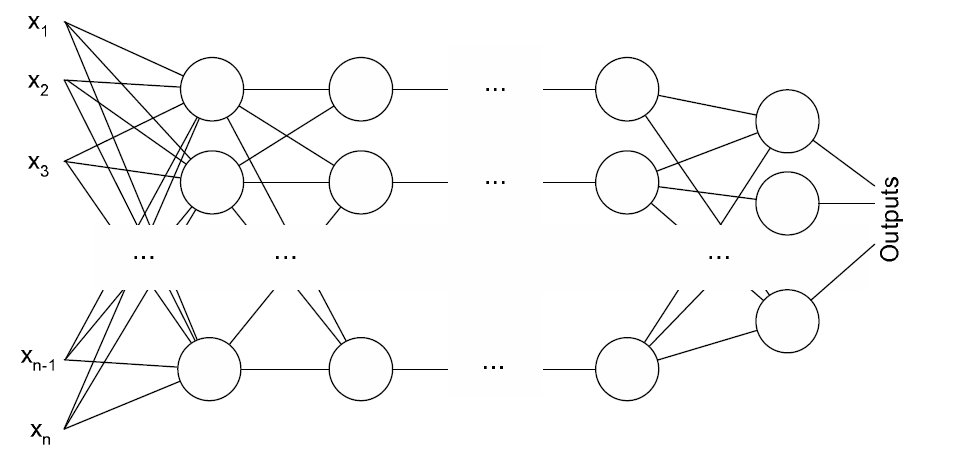
\includegraphics[width=0.7\linewidth]{images/MLP}
	\caption{Многослойный перцептрон}
	\label{fig:mlp}
\end{figure}

Во время обработки данные последовательно передаются от входа к выходу без использования сторонних циклов или обратной связи. Обучение полносвязных сетей выполняется при помощи алгоритма обратного распространения ошибки, используемого вместе с параллельным спуском.  Эти нейронные сети позволяют аппроксимировать и приближать практически любые непрерывные функции. Недостатками данной модели является плохая масштабируемость на задачи с большими входными данными, а также большие временные затраты на обучение, что делает ее непригодной для работы с изображениями.

Рекуррентная нейронная сеть разработана для работы с последовательными данными, например текстом, аудиосигналами. Отличительной чертой этого типа является наличие внутренней памяти, позволяющей учитывать контекст предыдущих вычислений при обработке новых данных. Базовой архитектурой рекуррентной сети является сеть входных, скрытых и выходных узлов, каждый из которых соединен с остальными. На вход каждого шага вместе с входными данными подается результат обработки предыдущего шага, что позволяет моделировать временные зависимости. Из-за этого метода обработки данных могут возникать проблемы с исчезновением или взрывом градиента ошибки, что было решено при разработке усовершенствованной сети с долгой краткосрочной памятью, LTSM. LTSM является сетью с ячейками памяти, позволяющими сохранять информацию на длительные промежутки времени. Обычно формируется с использованием <<вентилей>>, использующихся для контроля информации на входах и выходах памяти блоков.

\begin{figure}[h]
	\centering
	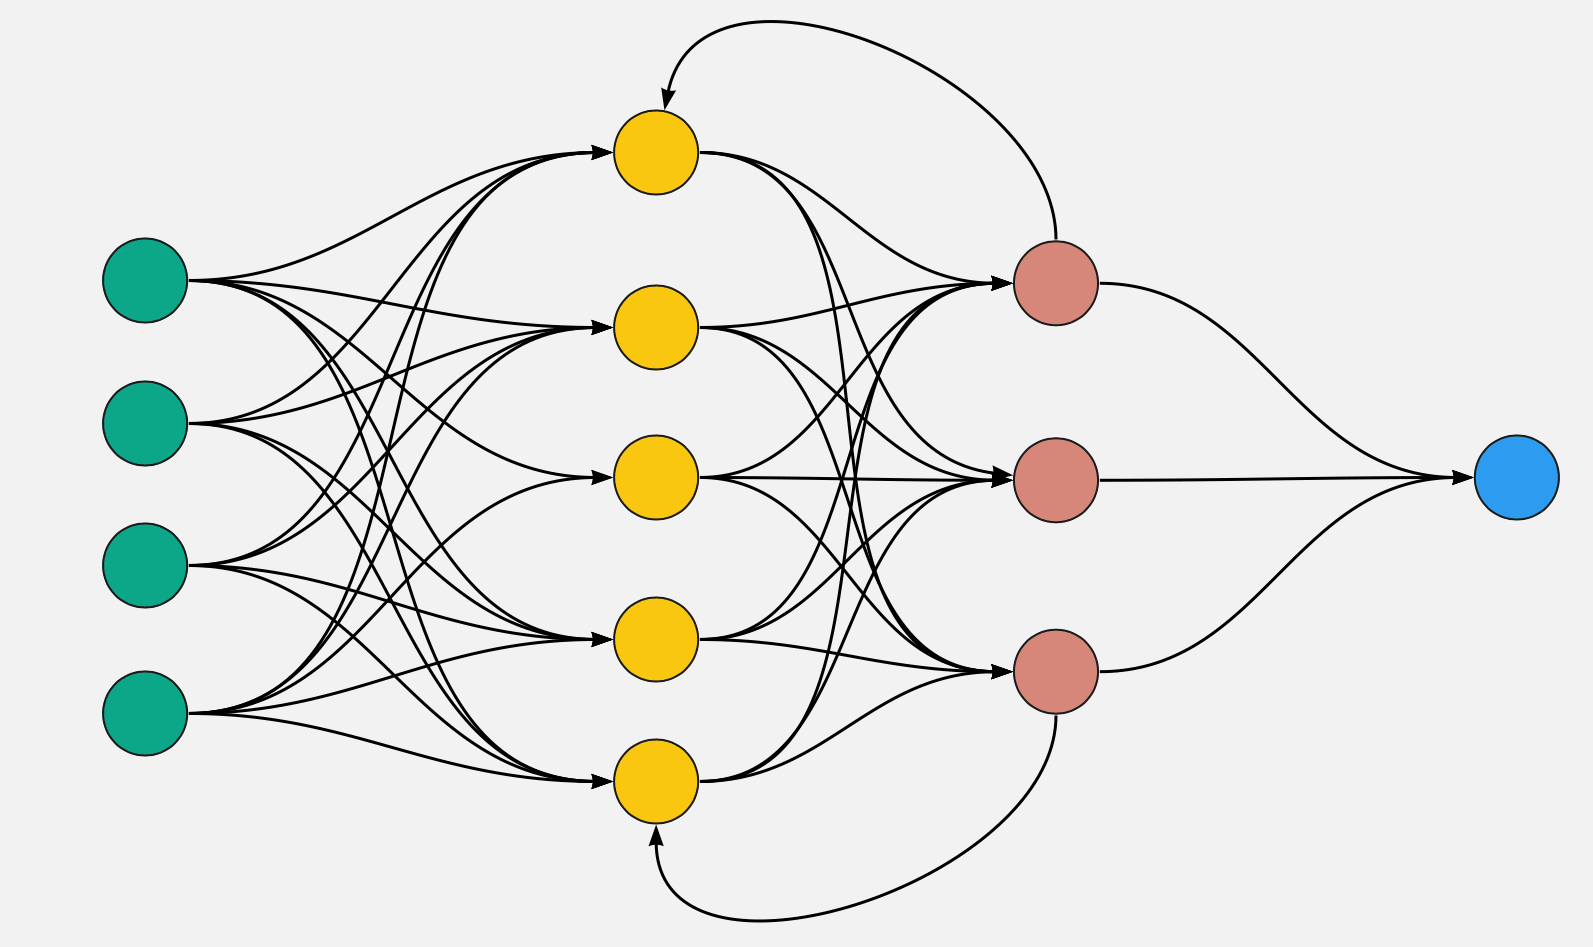
\includegraphics[width=0.7\linewidth]{images/RNN}
	\caption{Рекуррентная нейронная сеть}
	\label{fig:rnn}
\end{figure}

Сверточная нейронная сеть -- однонаправленная многослойная сеть, направленная на распознавание образов.

\begin{figure}[h]
	\centering
	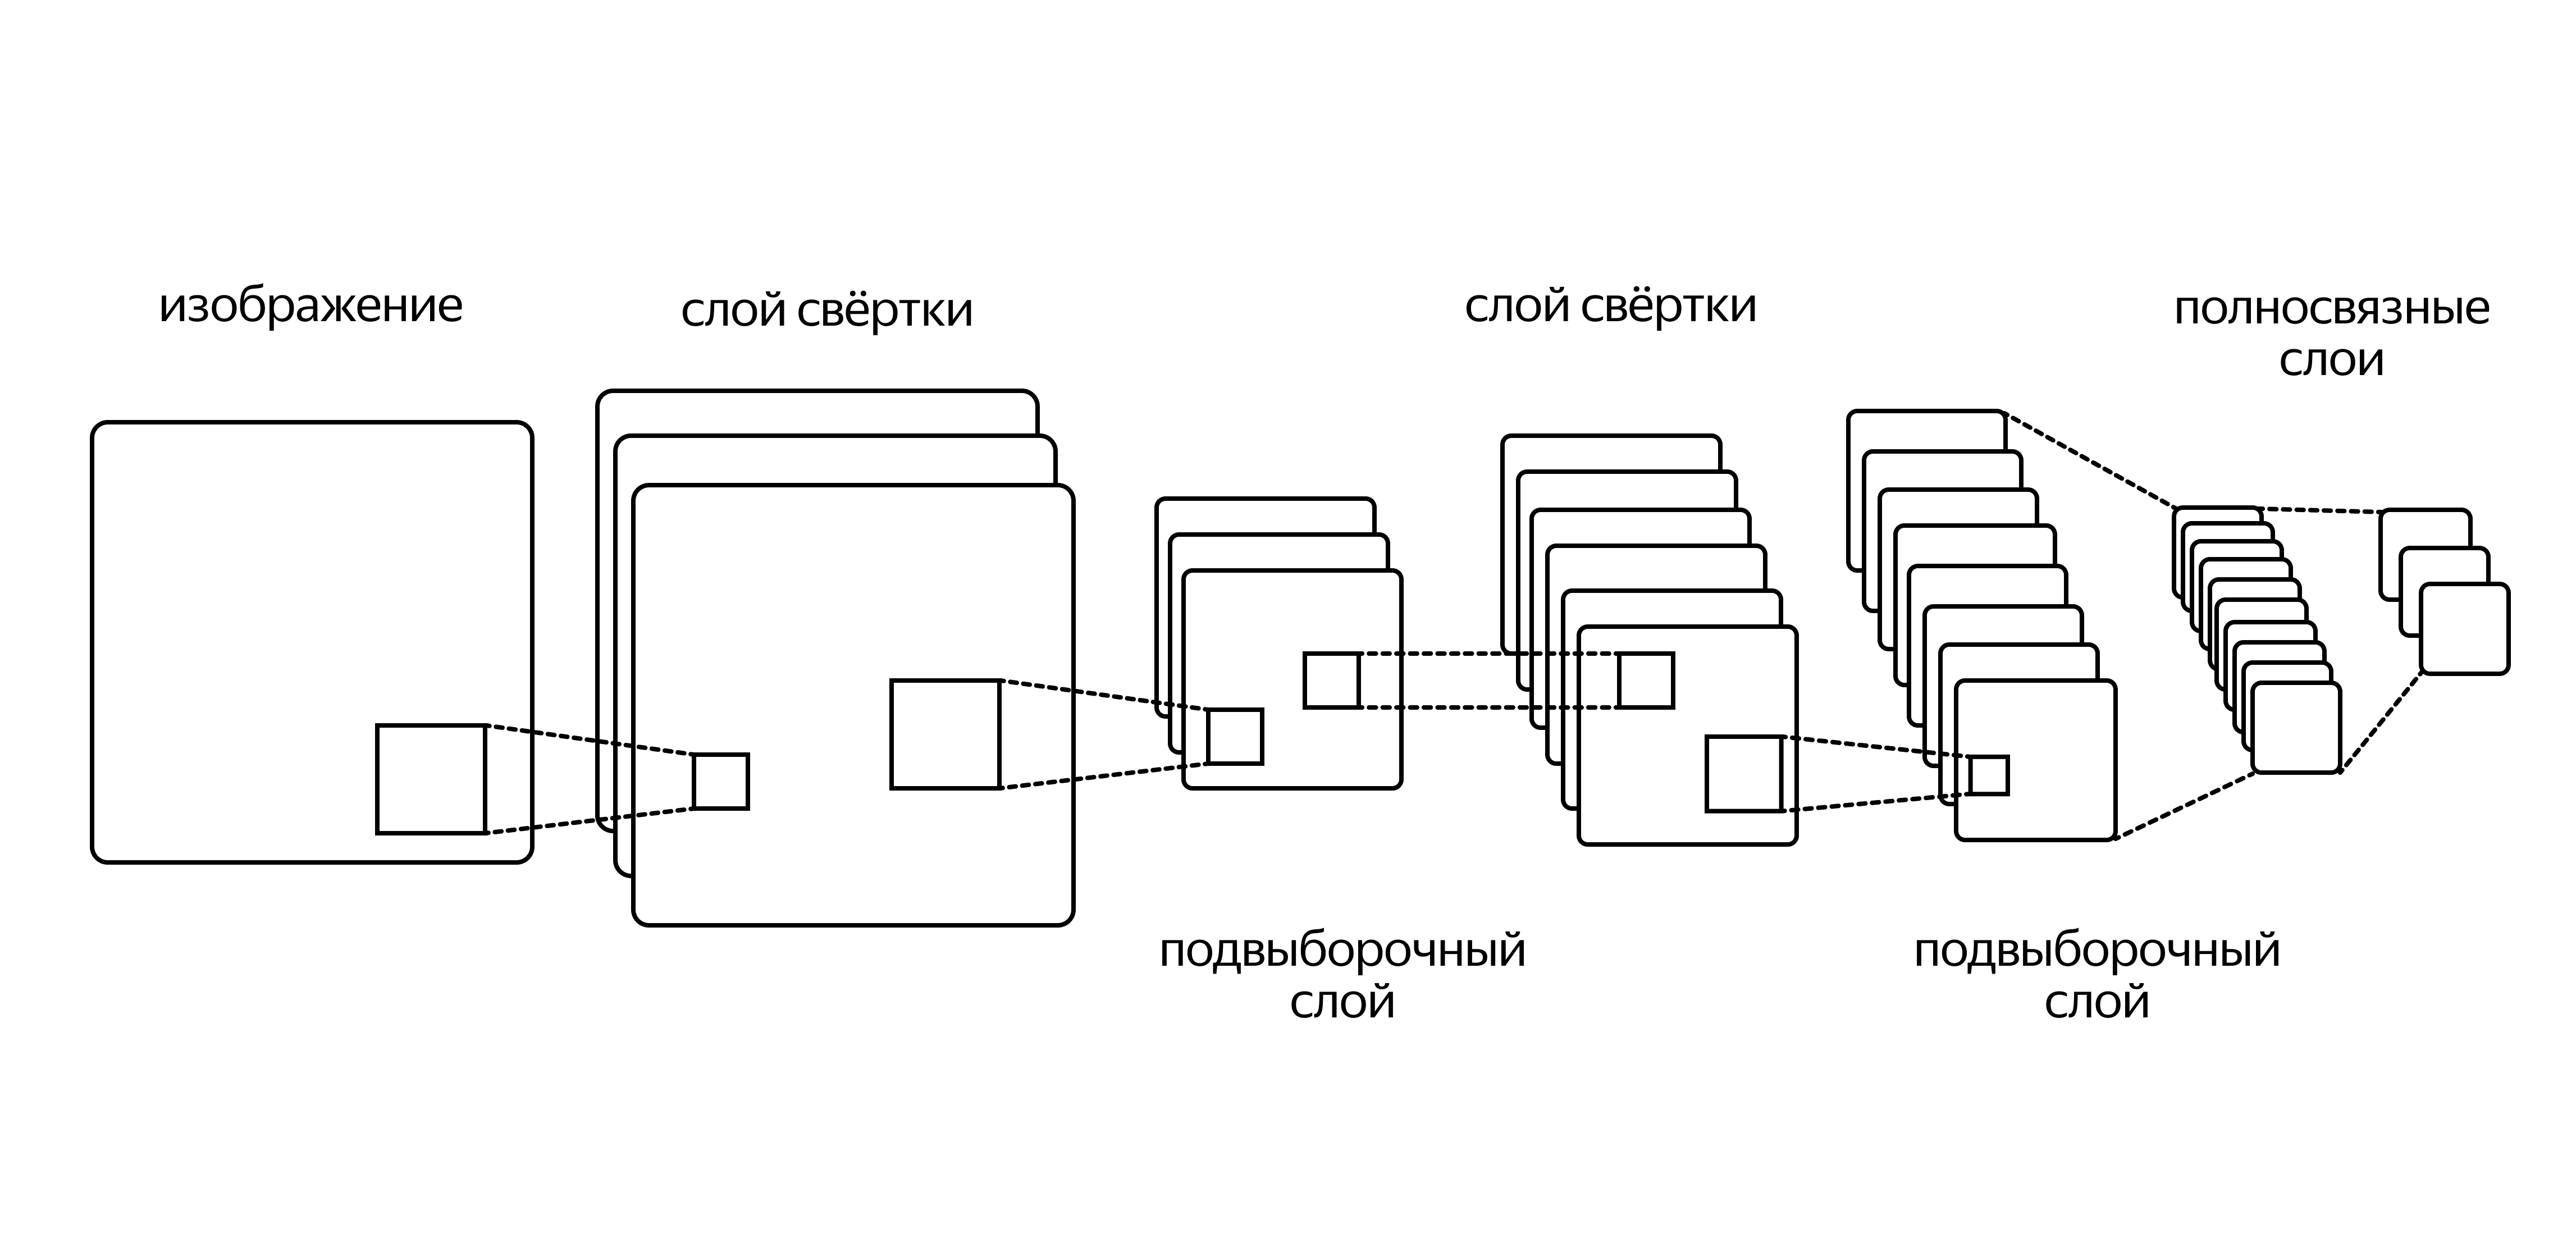
\includegraphics[width=0.7\linewidth]{images/CNN}
	\caption{Сверточная нейронная сеть}
	\label{fig:cnn}
\end{figure}

 Основным отличием от полносвязных сетей является использование сверточных слоев, применяющих одинаковые фильтры, называемые ядрами свертки. Эти ядра являются матрицами весов и последовательно перемещаются по обрабатываемому слою, вычисляя локальную свертку -- взвешенную сумму значений в пределах области матрицы, тем самым вычисляя локальные признаки. На выходе каждого фильтра формируется карта признаков, отражающая степень активации конкретного признака на различных участках слоя. Сверточные слои обычно чередуются с слоями подвыборки, сжимающими полученные карты признаков, выделяя и сохраняя наибольшее значение из конкретной небольшой области. После нескольких сверточных и подвыборочных слоев карты признаков передаются на полносвязные слои, обрабатывающие полученные данные. Сверточные нейронные сети чаще всего используются для обработки изображений, в частности задач сегментации. 
